\section{Processi primari}
\label{sec:Processi_Primari}
I processi primari definiti dalla norma \glossario{ISO/IEC 12207} sono essenziali per la realizzazione di un progetto e sono strettamente legati all'acquisizione, alla realizzazione, alla gestione, all'operazione e al ritiro del software durante l'intero ciclo di vita. 
Un processo primario consiste in un insieme di attività fondamentali e interconnesse, e variano a seconda della tipologia di processo.
Questi processi sono cruciali nelle fasi operative del ciclo di vita del software e sono determinanti per garantire una produzione, manutenzione e dismissione in modo efficace. La norma distingue cinque principali processi primari, ognuno dei quali comprende attività chiave per lo sviluppo e la gestione del software, dalla sua concezione fino al suo ritiro.
I cinque processi sono:
\begin{enumerate}
    \item \textbf{Processo di acquisizione}; 
    \item \textbf{Processo di fornitura}; 
    \item \textbf{Processo di sviluppo};
    \item \textbf{Processo di operazione}; 
    \item \textbf{Processo di manutenzione};
\end{enumerate}
\textbf{Nota bene}: Per la questione didattica il processo di manutenzione non verrà implementata.

\subsection{Processo di acquisizione}
\label{subsection:Processo_acquisizione}
Il processo di acquisizione, secondo la norma ISO/IEC 12207, comprende l'insieme delle attività che un'organizzazione, cioè il \glossario{Fornitore}, deve svolgere per ottenere un sistema, un prodotto software o un servizio software. Esso prevede l'identificazione dei requisiti, la selezione di un Fornitore e un \glossario{Proponente}, la stipula di un contratto, la supervisione della fornitura e, infine, l'accettazione e il completamento del prodotto o servizio acquisito.
Dunque, per il nostro gruppo, il processo di acquisizione consiste nelle seguenti attività principali:

\begin{itemize}
    \item \textbf{Iniziazione}; 
    \item \textbf{Studio di fattibilità}; 
    \item \textbf{Selezione del capitolato}; 
    \item \textbf{Preparazione della candidatura}; 
    \item \textbf{Accettazione della candidatura}; 
\end{itemize}

\subsubsection{Iniziazione}
Il Fornitore effettua un'analisi preliminare dei capitolati d’appalto, la comprensione degli obiettivi e dei requisiti iniziali per lo sviluppo, includendo il confronto e la discussione con i proponenti.

\subsubsection{Studio di fattibilità}
Il Fornitore analizza i capitolati per identificare eventuali punti critici e valuta le idee ricevute dai proponenti.

\subsubsection{Selezione del capitolato}
Il Fornitore sceglie e prepara il capitolato d'appalto che meglio soddisfa le sue aspettative.

\subsubsection{Preparazione della candidatura}
Il Fornitore prepara e definisce la redazione dei documenti necessari:
\begin{itemize}
    \item \textbf{Lettera di candidatura};
    \item \textbf{Stima dei costi};
    \item \textbf{Assunzione d’impegni};
    \item \textbf{Valutazione dei capitolati}.
\end{itemize}
Revisionando il contenuto per correggere eventuali errori e, se necessario, aggiorna il documento prima della presentazione ai \glossario{Committenti}.

\subsubsection{Accettazione della candidatura}
L'approvazione della soluzione selezionata e la conseguente formalizzazione del contratto spettano ai committenti, i quali, con la loro approvazione, rendono ufficiale il contratto.

\subsection{Processo di fornitura}
\label{subsection:processo_fornitura}
Il processo di fornitura, definito dalla norma ISO/IEC 12207, comprende le attività svolte dal Fornitore e inizia con la presentazione di una proposta al Proponente o la stipula di un contratto. Nel nostro caso, il processo riguarda la Proponente Zucchetti S.p.A. e si avvia al termine del processo di acquisizione, ossia al completamento della fase di accettazione della candidatura.
Il processo prevede la pianificazione e l’organizzazione delle risorse, delle procedure e dei piani necessari per la gestione del progetto, fino alla consegna del sistema, prodotto o servizio software. Questo processo è fondamentale per garantire che il software soddisfi i requisiti del cliente, sia di alta qualità e venga realizzato rispettando tempi e costi concordati. L’obiettivo principale è allineare costantemente le aspettative dell’acquirente con i risultati ottenuti durante l’esecuzione del progetto.
Dunque, per il nostro gruppo, il processo si articola nelle seguenti attività principali:
\begin{itemize}
    \item \textbf{Pianificazione};
    \item \textbf{Esecuzione e controllo};
    \item \textbf{Revisione e valutazione};
    \item \textbf{Consegna e completamento};
\end{itemize}

\subsubsection{Pianificazione}
Il Fornitore definisce obiettivi, risorse e procedure necessari per l’esecuzione del progetto, identificando i requisiti per la gestione, la misurazione della qualità e lo svolgimento delle attività. Questa fase sta principalmente nella redazione del Piano di Progetto, che pianifica l’utilizzo delle risorse e documenta i risultati attesi.

\subsubsection{Esecuzione e controllo}
Il Fornitore attua le attività pianificate nel Piano di Progetto, rispettando le norme stabilite. Inoltre, viene effettuato un controllo continuo sullo stato di avanzamento e sulla gestione delle risorse, garantendo la rendicontazione rispetto agli obiettivi prefissati. 

\subsubsection{Revisione e valutazione}
Il Fornitore definisce criteri e procedure per la revisione ed esegue le operazioni in conformità a tali criteri. L'obiettivo è verificare che il progetto soddisfi i requisiti e rispetti gli standard stabiliti.

\subsubsection{Consegna e completamento}
Consegna del progetto, verifica finale e accettazione da parte dell’acquirente.

\subsubsection{Contatti con la Proponente dell’azienda}
La Proponente, Zucchetti S.p.A., fornisce l'indirizzo email del proprio rappresentante per la comunicazione asincrona e per la pianificazione di videochiamate su Google Meet con il Fornitore. Le comunicazioni tra Proponente e Fornitore riguardano vari aspetti del progetto, tra cui la raccolta dei requisiti, la raccolta di feedback sui risultati ottenuti e le indicazioni sull'avanzamento del progetto. Durante il corso del progetto, che ha carattere didattico, la Proponente assume il ruolo di cliente, mantenendo un ampio grado di libertà per il Fornitore, il quale è responsabile della realizzazione del prodotto. Per ogni colloquio con l'azienda Proponente, ovvero per ogni videochiamata tramite Google Meet, sarà redatto un Verbale Esterno che riassume i punti chiave discussi durante l'incontro.

\subsubsection{Documentazione fornita}
Di seguito viene descritta la documentazione che il gruppo rende disponibile alla Proponente Zucchetti S.p.A. e ai committenti, Prof. Tullio Vardanega e Prof. Riccardo Cardin.

\paragraph{Piano di progetto}
Il Piano di Progetto è un documento redatto dal responsabile del progetto, che fornisce una visione dettagliata della gestione e dell’organizzazione del gruppo di lavoro. La sua funzione principale è quella di pianificazione, monitoraggio e controllo delle attività, al fine di garantire il raggiungimento degli obiettivi nei tempi e nei costi stabiliti. Inoltre, il piano include l'analisi e la gestione dei rischi, nonché la pianificazione, il preventivo e il consuntivo di ciascun sprint, monitorando costantemente l'avanzamento del progetto e le risorse utilizzate.
Il documento è suddiviso nelle seguenti sezioni:
\begin{itemize}
    \item \textbf{Introduzione}: Una breve descrizione dello scopo del documento e delle varie sezioni che lo compongono.
    \item \textbf{Analisi dei rischi}: Riguarda l'identificazione dei potenziali rischi che potrebbero sorgere durante il corso del progetto, i quali potrebbero causare ritardi o ostacoli nella sua progressione. Vengono inoltre sviluppate strategie di prevenzione per evitare che tali rischi si manifestino, nonché strategie di mitigazione per ridurne l'impatto nel caso in cui si verificassero, al fine di garantire la continuità del progetto.
    \item \textbf{Stima dei costi}: Calcolo delle risorse necessarie per il completamento del progetto, che viene aggiornato ad ogni sprint.
    \item \textbf{\glossario{Milestone} principali}: Sezione dedicata all'indicazione delle milestone fondamentali e delle baseline di riferimento del progetto.
    \item \textbf{Primo periodo}: Rappresenta la fase iniziale del gruppo.
    \item \textbf{\glossario{Sprint}}: Gli sprint rappresentano fasi del progetto in cui vengono definiti obiettivi specifici e attività da completare. Durante ogni sprint, il gruppo si impegna a raggiungere tali obiettivi. Inoltre, si stabiliscono una revisione retrospettiva e la data per lo sprint successivo.
    La sottosezione si articola nelle seguenti parti:
    \begin{enumerate}
        \item \textbf{Obiettivi}: Definisce gli obiettivi specifici dello sprint.
        \item \textbf{Pianificazione}: Presenta il preventivo dei costi e delle risorse previste per lo sprint.
        \item \textbf{Consuntivo}: Riporta il resoconto dei costi e delle risorse effettivamente utilizzati.
        \item \textbf{Retrospettiva}: Riporta la conclusione dello sprint e propone miglioramenti sui punti deboli emersi.
        \item \textbf{Aggiornamento risorse rimaste}: Aggiorna la situazione delle risorse disponibili per il progetto.
    \end{enumerate}
\end{itemize}

\paragraph{Analisi dei requisiti}
L’analisi dei requisiti è un documento redatto dall’analista che fornisce una visione chiara delle richieste e delle aspettative dell’azienda Proponente. Va ad includere un elenco dettagliato delle funzionalità da sviluppare e implementare, nonché i casi d’uso che definiscono le interazioni tra il sistema e l’utente.
Il documento è suddiviso nelle seguenti sezioni:
\begin{enumerate}
    \item \textbf{Introduzione}: Una breve descrizione dello scopo del documento e delle varie sezioni che lo compongono.
    \item \textbf{Descrizione del prodotto}: Descrive gli obiettivi del prodotto, le sue funzioni principali e le caratteristiche.
    \item \textbf{Casi d’uso}: Indica tutti i casi d’uso individuati dal gruppo durante analisi.
    \item \textbf{Requisiti}: Elenco completo dei requisiti del prodotto, organizzato per categorie e con riferimento alle fonti da cui proviene il tracciamento.
\end{enumerate}

\paragraph{Piano di Qualifica}
Il Piano di Qualifica è un documento che definisce le attività del verificatore nel progetto, stabilendo le strategie e gli approcci per garantire la qualità del prodotto software in fase di sviluppo. Redatto dal verificatore, questo documento descrive le modalità di verifica e validazione. Tutti i membri del team si baseranno su questo documento per garantire il raggiungimento della qualità desiderata.
Il documento è suddiviso nelle seguenti sezioni: 
\begin{enumerate}
    \item \textbf{Introduzione}: Una breve descrizione dello scopo del documento e delle varie sezioni che lo compongono.
    %\item \textbf{Obiettivi di qualità}: Questa sezione presenta i valori accettabili e gli ambiti per le metriche definite dal team, le metriche sono divise:Qualità di processo,Qualità di prodotto,Qualità per obiettivo.
    %\item \textbf{Metodologie di testing}: Include tutti i test necessari per verificare che il prodotto rispetti i requisiti specificati.
    %\item \textbf{Cruscotto di valutazione della qualità}: Vengono scritte tutte le attività di verifica effettuate e le problematiche emerse durante lo sviluppo del software.
\end{enumerate}

\paragraph{Glossario}
Il Glossario è un elenco dettagliato e organizzato di tutti termini, acronimi e definizioni utilizzati nella documentazione. L’obiettivo principale di questo documento è fornire una comprensione chiara dei concetti e dei termini specifici impiegati nel progetto, garantendo una comunicazione coerente e precisa tra tutti i membri del gruppo e con gli \glossario{Stakeholder}. In questo modo, si facilita il lavoro collaborativo e si assicura un allineamento efficace su linguaggio e significati durante l'intero ciclo di vita del progetto.

\paragraph{Lettera di presentazione}
La Lettera di Presentazione è il documento con cui il gruppo comunica la propria candidatura alle revisioni di avanzamento \glossario{Requirements and Technology Baseline} e \glossario{Product Baseline}. Nel primo caso essa include informazioni sui repository di documentazione e codice sorgente, il riferimento al \glossario{Proof of Concept} e un aggiornamento sugli impegni con la stima del preventivo "a finire". 

\subsection{Processo di sviluppo}
\label{subsection:processo_sviluppo}
ll processo di sviluppo riguarda l'insieme di attività necessarie per produrre e implementare il software, assicurandosi che risponda ai requisiti definiti e sia di qualità adeguata.

\subsubsection{Analisi dei requisiti}
L'analisi dei requisiti è una attività cruciale nel ciclo di vita del software, in cui vengono raccolte, analizzate e documentate le esigenze degli stakeholder per definire chiaramente cosa il sistema dovrà fare. 
Questa attività produce il documento di analisi dei requisiti descritto nella sezione \hyperref[subsec:documentazione]{Documentazione}.

\paragraph{Requisiti}
I requisiti vengono categorizzati in:
\begin{enumerate}
    \item \textbf{Requisiti funzionali}.
    
    Rappresentano ciò che un sistema deve fare per soddisfare le esigenze degli utenti o degli stakeholders.

    \item \textbf{Requisiti qualitativi}.
    
    I requisiti di qualità (requisiti non funzionali) descrivono caratteristiche qualitative del sistema, come prestazioni, sicurezza, usabilità e manutenibilità.

    \item \textbf{Di vincolo}.
    
    I requisiti di vincolo rappresentano limitazioni o condizioni obbligatorie che influenzano lo sviluppo, l'implementazione o l'operatività del sistema. 
    A differenza dei requisiti funzionali o di qualità, non descrivono cosa deve fare il sistema, ma come deve essere realizzato rispettando regole o restrizioni specifiche. 

    \item \textbf{Prestazionali}.
    
    I requisiti prestazionali sono un tipo specifico di requisiti non funzionali che definiscono le aspettative relative alle prestazioni del sistema.
    Alcuni esempi sono: la velocità, il tempo di risposta, la capacità di carico, e altre caratteristiche misurabili legate all'efficienza.
\end{enumerate}


\paragraph{Casi d'uso}
I casi d'uso forniscono una descrizione dettagliata delle funzionalità del sistema dal punto di vista degli utenti, delineando come il sistema risponda a specifiche azioni o scenari. 
In particolare un caso d'uso rappresenta un uso completo del sistema dalla prospettiva dell'utente.
I casi d'uso vengono rappresentati tramite una combinazione di descrizione e diagramma UML.
Durante la definizione di un caso d'uso possono emergere nuove informazioni che richiedono una modifica dei casi d'uso definiti in precedenza.
La definizione dei casi d'uso non è quindi lineare.

\subparagraph{Descrizione}
Nella \hyperref[tab:template_casi_uso]{Tabella \ref{tab:template_casi_uso}} viene mostrato il template per la descrizione dei casi d'uso.
Ogni descrizione di caso d'uso deve includere:
\begin{enumerate}
    \item \textbf{Identificativo}.
    
    \texttt{UC-<ID caso principale>.<ID sotto caso>}. 
    
    Dove:
    \begin{enumerate}
        \item \texttt{<ID caso principale>}: identificativo numerico del caso d'uso principale (numero crescente).

        \item \texttt{<ID sotto caso>}: identificativo numerico del sotto caso d'uso (presente solo se si tratta di un sotto caso d'uso).
    \end{enumerate}

    \item \textbf{Pre-condizioni}.
    
    Stato iniziale del sistema o vincoli necessari per l'attivazione del caso d'uso.

    \item \textbf{Post-condizioni}.
    
    Stato finale del sistema dopo un esecuzione normale(priva di errori) del caso d'uso.

    \item \textbf{Post-condizioni errore}.
    
    Stato finale del sistema dopo un esecuzione fallita del caso d'uso.

    \item \textbf{Attori}.
    Un attore è un entità esterna(\underline{umana o meno}) al sistema che interagisce con il sistema per iniziare o per contribuire al compimento l'esecuzione di un caso d'uso.  
    Gli attori si dividono in:
    \begin{enumerate}
        \item  \textbf{Attori primari}: attori principali che partecipano al caso d'uso, solitamente contengono gli attori che iniziano l'interazione e/o sono i destinatari delle informazioni in output del caso d'uso.
        \item \textbf{Attore secondario}: altri attori coinvolti che non sono protagonisti nell'esecuzione del caso d'uso(es. Sistemi esterni).
    \end{enumerate}

    \item \textbf{Trigger}.
    
    Evento eseguito da un attore che attiva il caso d'uso.
    
    \item \textbf{User story}.
    
    Una breve descrizione di una funzionalità del software, scritta dal punto di vista dell'utente, che fornisce contesto, obiettivi e valore.
    L'user story viene scritta nella forma:
    \begin{center}
        \small
        \texttt{\textit{"Come <utente> desidero poter <funzionalità> per <valore aggiunto>"}}.
    \end{center}

    \item \textbf{Scenario principale}.
    
    La sequenza di step importanti che vengono portati a termine in un esecuzione normale del caso d'uso.
    
    \item \textbf{Scenario alternativo}.

    Eventuali deviazioni o eccezioni rispetto allo scenario principale.
\end{enumerate}

\begin{table}[H]
    \resizebox{\textwidth}{!}{
    \begin{tabular}{l l l}
       
            \rowcolor{lightgray}
            \textbf{Nome caso d'uso} & & \texttt{\textbf{<identificativo caso d'uso>}} \\ 

            Pre-condizioni & & \texttt{<pre-condizioni>} \\
            Post-condizioni & & \texttt{<post-condizioni>} \\
            Post-condizioni errore & & \texttt{<post-condizioni errore>} \\
            Attori principali & & \texttt{<lista attori principali>} \\
            Attori secondari & & \texttt{<lista attori secondari>} \\
            Trigger & & \texttt{<trigger>} \\
            Casi d'uso inclusi & & \texttt{<lista casi d'uso inclusi>}\\
            Caso d'uso base & & \texttt{<caso d'uso di base>}\\
            Scenario principale & \textbf{Step} & \textbf{Azione} \\
            & 1 & \texttt{<$1^a$ azione>} \\
            & \texttt{\textbf{include::<nome caso d'uso>}} & \\
            & 2 & \texttt{<$2^a$ azione>} \\
            & ... & ... \\
            Estensioni & \textbf{Step} & \textbf{Azione alternativa} \\ 
            & 2.1 & \texttt{<$1^a$ azione a partire dal $2^o$ step>} \\
            & 2.2 & \texttt{<$2^a$ azione a partire dal $2^o$ step>} \\
            & ... & ... \\
    \end{tabular}}
    \caption{Template tabella dei casi d'uso.}
    \label{tab:template_casi_uso}
\end{table}

\subparagraph{Diagrammi dei casi d'uso}
I diagrammi dei casi d'uso sono strumenti grafici utilizzati nell'ingegneria del software per rappresentare in modo intuitivo le interazioni tra gli utenti (attori) e un sistema. Basati sul linguaggio UML (Unified Modeling Language), questi diagrammi illustrano i principali scenari operativi del sistema e aiutano a identificare e chiarire i requisiti funzionali.
Ogni diagramma è composto da:
\begin{itemize}
    \item \textbf{Sistema}: delimita i confini del sistema software, indicando quali funzionalità sono incluse e quali sono esterne a esso.
    Il sistema viene rappresentato nei diagrammi come mostrato in \hyperref[fig:sistema_uml]{Figura \ref{fig:sistema_uml}}.
    \begin{figure}[H]
        \centering
        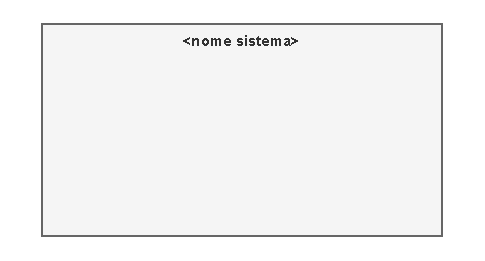
\includegraphics{Sezioni/ProcessiPrimari/Immagini/sistema_caso_uso.pdf}
        \caption{Rappresentazione del sistema in UML.}
        \label{fig:sistema_uml}
    \end{figure}
    
    \item \textbf{Attori}: rappresentano soggetti che interagiscono con il sistema software. Gli attori possono essere persone, altri applicativi o dispositivi che utilizzano le funzionalità del sistema.
    Un attore viene rappresentato nei diagrammi usando una delle due notazioni mostrate in \hyperref[fig:attori_uml]{Figura \ref{fig:attori_uml}} posta al di fuori del sistema.
    \begin{figure}[H]
        \centering
        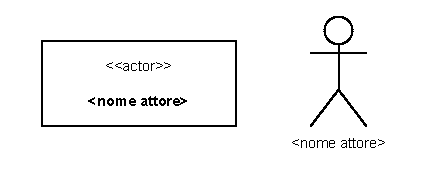
\includegraphics{Sezioni/ProcessiPrimari/Immagini/attori_caso_uso.pdf}
        \caption{Rappresentazione degli attori in UML.}
        \label{fig:attori_uml}
    \end{figure}
    
    \item \textbf{Casi d'uso}: rappresentano le funzionalità o i servizi offerti dal sistema che producono un risultato di valore per un attore. Ogni caso d'uso descrive una sequenza specifica di interazioni tra gli attori e il sistema.
    Ogni caso d'uso viene rappresentato nei diagrammi usando la notazione mostrata in \hyperref[fig:caso_uso]{Figura \ref{fig:caso_uso}} posta all'interno del sistema.
    \begin{figure}[H]
        \centering
        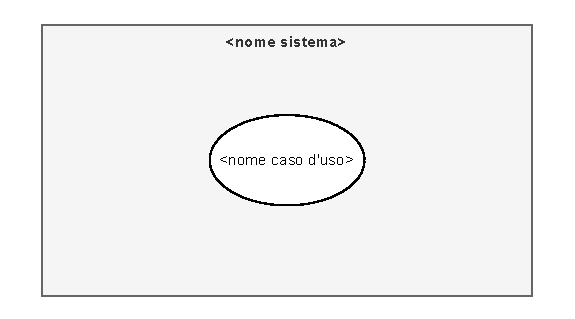
\includegraphics{Sezioni/ProcessiPrimari/Immagini/caso_uso.pdf}
        \caption{Rappresentazione caso d'uso in UML.}
        \label{fig:caso_uso}
    \end{figure}
    
    \item \textbf{Relazioni}.
    
    Sono delle notazioni che permettono di rendere più modulari i diagrammi di casi d'uso e di rendere chiara l'interazione degli attori con il sistema.
    
    \begin{itemize}
        \item \textbf{Associazione}: è la relazione fondamentale che collega un attore a un caso d'uso a cui esso partecipa.
        Uno stesso attore può partecipare a \texttt{N} casi d'uso.
        Le associazioni vengono rappresentate in UML come mostrato in \hyperref[fig:associazione_uml]{Figura \ref{fig:associazione_uml}}.
        \begin{figure}[H]
            \centering
            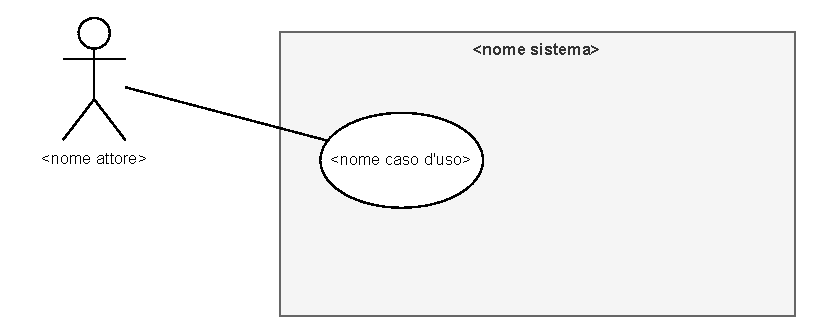
\includegraphics{Sezioni/ProcessiPrimari/Immagini/associazione_uml.pdf}
            \caption{Rappresentazione associazione in UML.}
            \label{fig:associazione_uml}
        \end{figure}

        \item \textbf{Inclusione}: rappresenta una dipendenza in cui il comportamento del caso d'uso incluso è incorporato ogni volta che viene eseguito il caso d'uso base. Il caso d'uso incluso contiene funzionalità che sono riutilizzate in più casi d'uso principali, permettendo di evitare la duplicazione di comportamenti comuni.
        L'inclusione viene rappresentata in UML come mostrato in \hyperref[fig:inclusione_uml]{Figura \ref{fig:inclusione_uml}}.
        \begin{figure}[H]
            \centering
            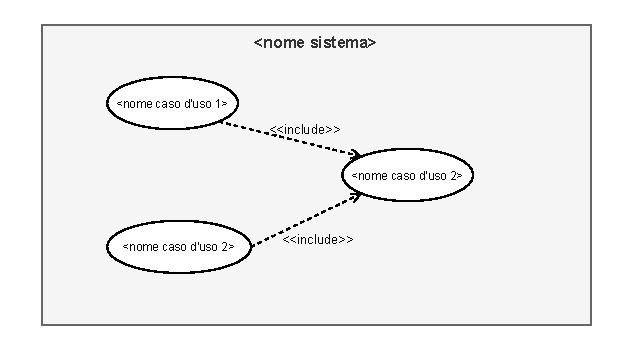
\includegraphics{Sezioni/ProcessiPrimari/Immagini/inclusione_uml.pdf}
            \caption{Rappresentazione inclusione in UML.}
            \label{fig:inclusione_uml}
        \end{figure}
        Come si può vedere nella \hyperref[tab:template_casi_uso]{Tabella \ref{tab:template_casi_uso}} è necessario:
        \begin{enumerate}
            \item Indicare il caso d'uso incluso come valore della colonna "Casi d'uso inclusi".
            \item Indicare lo step dello scenario principale o delle estensioni che utilizza il caso d'uso incluso.
            Questo viene fatto tramite la sintassi \texttt{include::<nome caso d'uso>}.
        \end{enumerate} 

        \item \textbf{Estensione}: mostra una relazione in cui un caso d'uso esteso aumenta le funzionalità del caso d'uso principale. Il caso d'uso esteso viene eseguito solo sotto determinate condizioni, interrompendo l'esecuzione del caso d'uso principale.
        L'estensione viene rappresentata in UML come mostrato in \hyperref[fig:estensione_uml]{Figura \ref{fig:estensione_uml}}.
        \begin{figure}[H]
            \centering
            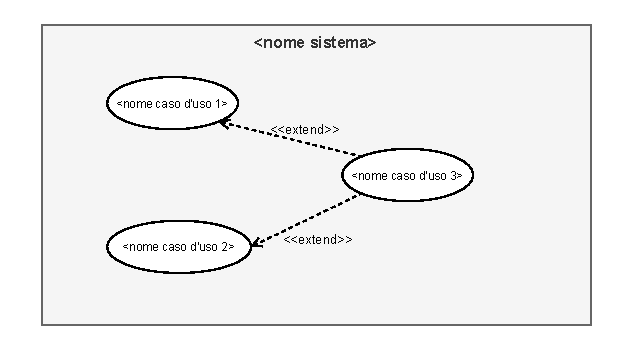
\includegraphics{Sezioni/ProcessiPrimari/Immagini/estensione_uml.pdf}
            \caption{Rappresentazione estensione in UML.}
            \label{fig:estensione_uml}
        \end{figure}
        
        \item \textbf{Generalizzazione}: rappresenta una relazione in cui un caso d'uso figlio può aggiungere funzionalità o modificare il comportamento di un caso d'uso genitore. Tutte le funzionalità definite nel caso d'uso genitore si mantengono nel caso d'uso figlio se queste non vengono ridefinite.
        La generalizzazione viene rappresentata in UML come mostrato in \hyperref[fig:generalizzazione_uml]{Figura \ref{fig:generalizzazione_uml}}.
        \begin{figure}[H]
            \centering
            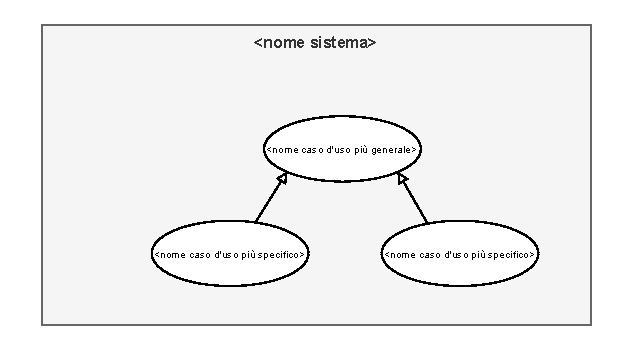
\includegraphics{Sezioni/ProcessiPrimari/Immagini/generalizzazione_uml.pdf}
            \caption{Rappresentazione generalizzazione in UML.}
            \label{fig:generalizzazione_uml}
        \end{figure}
        Come si può vedere nella \hyperref[tab:template_casi_uso]{Tabella \ref{tab:template_casi_uso}} è necessario indicare il caso d'uso genitore come valore della colonna "Caso d'uso base".

    \end{itemize}

    \item \textbf{Sottocasi d'uso}: i sottocasi d'uso rappresentano scenari specifici e dettagliati che si sviluppano all'interno di un caso d'uso principale. La loro funzione è di descrivere in modo approfondito le diverse situazioni o varianti operative che possono verificarsi nel contesto del caso d'uso generale.
    In particolare, ogni caso d'uso può essere suddiviso in più sottocasi, ciascuno associato a una specifica pagina o componente funzionale correlata al caso d'uso principale.
    
\end{itemize}

\paragraph{Fonti per l'Individuazione dei Casi d'Uso}
L'individuazione dei casi d'uso si basa principalmente sul capitolato fornito, che rappresenta una fonte essenziale per comprendere le caratteristiche generali del software da realizzare. 
Il capitolato, descrive le funzionalità principali e gli obiettivi del sistema, specificando alcuni requisiti chiave. 

Tuttavia, non tutti gli aspetti operativi sono dettagliati nel documento, il che rende necessaria un'integrazione attraverso deduzioni basate su necessità logiche e conoscenze pregresse. 
Il capitolato guida l'identificazione delle macro interazioni, consentendo di delineare i casi d'uso principali e il contesto generale in cui il sistema opererà. 
Tuttavia, nei punti in cui le specifiche risultano incomplete o generiche, è indispensabile adottare un approccio pro attivo, immaginando scenari d'uso che derivano dall'analisi delle esigenze tipiche di sistemi simili e delle best practices nel settore.

Questa attività di interpretazione si traduce nella definizione di ulteriori dettagli operativi, come eccezioni o varianti necessarie per garantire una piena copertura dei processi e un corretto funzionamento del sistema.

\subparagraph{Individuazione dei casi d'uso}
L'identificazione dei casi d'uso avviene attraverso i seguenti passaggi:
\begin{enumerate}
    \item \textbf{Identificazione degli attori}: Gli attori sono individuati in base ai loro ruoli e alle loro necessità operative. 
    Ad esempio, in un sistema gestionale possono essere individuati attori come l'amministratore, l'utente finale e un sistema di terze parti che si integra per la gestione dei pagamenti.
    L'identificazione degli attori è fondamentale per comprendere chi interagirà con il sistema e quali sono le operazioni che gli utenti devono poter eseguire.
    In \hyperref[fig:identificare_attori]{Figura \ref{fig:identificare_attori}} viene mostrata una tecnica utile per decidere se un concetto che appare nei requisiti è un attore o meno.
    \begin{figure}[H]
        \centering
        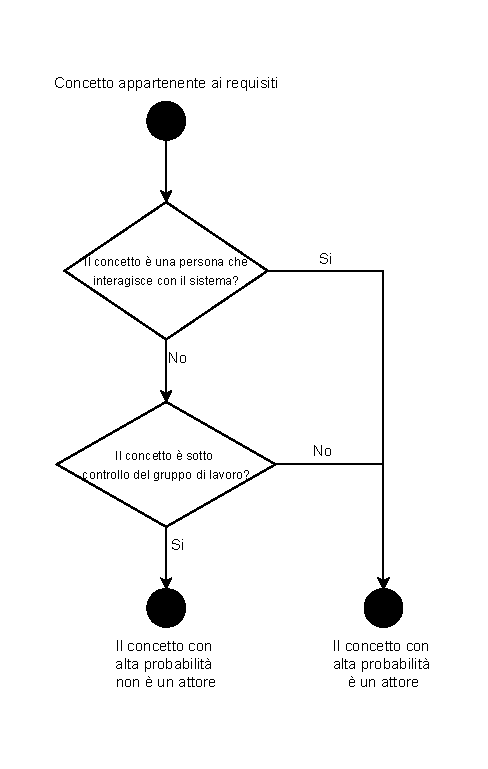
\includegraphics{Sezioni/ProcessiPrimari/Immagini/tecnica_casi_uso.pdf}
        \caption{Tecnica per identificare gli attori.}
        \label{fig:identificare_attori}
    \end{figure} 

    \item \textbf{Raffinamento attori}: Una coppia di attori può essere in una particolare relazione chiamata generalizzazione.
    In questa relazione l'attore "più generale" può eseguire un insieme di interazioni con il sistema che sono un sotto insieme delle interazioni che può eseguire l'attore "più specializzato".
    In altre parole l'attore "più specializzato" può eseguire tutte le interazioni che può eseguire l'attore "più generico" più eventuali ulteriori interazioni.
    In questo passaggio è importante scoprire queste relazioni tra gli attori.

    \item \textbf{Analisi degli obiettivi degli attori}: Una volta identificati gli attori e le relazioni tra essi, vengono analizzati i loro obiettivi in relazione al sistema. 
    Questo processo si basa sulla comprensione dei risultati che ogni attore desidera ottenere, come ad esempio la gestione di un ordine, l'accesso a report personalizzati o la possibilità di modificare parametri di configurazione.
    Gli obiettivi degli attori aiutano a delineare il perimetro dei casi d'uso e a definire le funzionalità che il sistema deve supportare per soddisfare tali obiettivi.

    \item \textbf{Identificazione dei casi d'uso principali}: Partendo dagli obiettivi individuati, si procede con la definizione dei casi d'uso principali. Questi rappresentano le macro funzionalità del sistema, cioè le interazioni essenziali e più frequenti tra gli attori e il sistema stesso. Ogni caso d'uso principale viene descritto in termini di azioni, e risultati attesi, garantendo che le funzionalità fondamentali siano chiaramente delineate.
    
    \item \textbf{Scomposizione in sotto-casi}: I casi d'uso principali possono venire successivamente scomposti in sotto-casi, se necessario, per dettagliare specifiche eccezioni, varianti o processi secondari. Questa scomposizione permette di descrivere scenari più specifici o complessi che possono verificarsi durante l'interazione. Ad esempio, il caso d'uso principale "Gestione di un ordine" può essere suddiviso nei sotto-casi "Modifica di un ordine esistente" e "Cancellazione di un ordine in attesa". Questo livello di dettaglio consente di rappresentare in modo accurato e completo tutti i comportamenti attesi del sistema.

\end{enumerate}